\documentclass{ijsra}
%----- will be part of version 0.5
\renewcommand\AD{{\,AD\xspace}}
\renewcommand\BC{{\,BC\xspace}}
%--------
\def\IJSRAidentifier{\currfilebase}%<<<< DO NOT change this line
\def\shorttitle{Elephant imagery on Greek coinage}
\def\maintitle{Local contexts to elephant imagery on Greco-Bactrian and Indo-Greek coinage}
\def\cmail{}
\def\keywords{Hellenistic, Greco-Bactrian, Indo-Greek, Numismatics, Royal Ideology, Elephants}
%\def\keywordname{}
\def\abstract{The \IJSRAsection{Abstract} monarchs of the Greco-Bactrian and Indo-Greek kingdoms in Hellenistic Bactria and India are known mainly through coins. This article studies the political significance of elephant motifs on Greco-Bactrian and Indo-Greek coinage. The study involves content and context analysis of the iconography in order to gain an understanding of the meaning and function of the elephant imagery. Through the analysis, the paper argues that Greco-Bactrian and Indo-Greek kings used elephant symbolism to express royal power in a cross-cultural context. Hellenocentric approaches that overlook the local context to royal power in Hellenistic kingdoms are challenged. This helps provide a clearer understanding of how Hellenistic kings established and maintained control over kingdoms with multiethnic populations.}
\def\authorone{Rahul Raza}
\undef\bioone%{\emph{Master's student?}}% needed
\def\affilone{Classical Archaeology, University of Oxford}


\begin{filecontents}{\IJSRAidentifier.bib}
@incollection{Abdullaev1995,
    author = {Abdullaev, K.},
    title = {Armour of ancient Bactria},
    pages = {163--180},
    editor = {Invernizzi, A.},
    booktitle = {In the land of the gryphons: papers on Central Asian archaeology in antiquity},
    publisher = {Le lettere},
    location = {Firenze},
    year = {1995},
    }

@book{Alter2004,
    author = {Alter, S.},
    title = {Elephas Maximus},
    publisher = {Harcourt},
    location = {Orlando},
    year = {2004},
    }

@incollection{Alonso2013,
    author = {Alonso Troncoso, V.},
    title = {The Diadochi and the zoology of kingship: The elephants},
    pages = {254--270},
    editor = {Alonso Troconso, V. and Anson, E.},
    booktitle = {After Alexander: The Time of the Diadochi (323-281 BC)},
    publisher = {Oxbow Books},
    location = {Oxford},
    year = {2013},
    }

@article{Bannikov2013,
   author = {Bannikov, A.V. and Popov, A.},
   title = {War elephants in Greco-Bactrian and Indo-Greek Armies},
   pages = {1206--1211},
   journaltitle = {World Applied Sciences Journal},
   volume = {27},
   year ={2013},    
    }

@book{Billows1995,
    author = {Billows, R.},
    title = {Kings and colonists: Aspects of Macedonian imperialism},
    publisher = {Brill},
    location = {Leiden},
    year = {1995},
    }

@book{Bopearachchi1991,
    author = {Bopearachchi, O.},
    title = {Monnaies gréco-bactriennes et indo-grecques: Catalogue raisonné},
    publisher = {Bibliothèque nationale},
    location = {Paris},
    year = {1991},
    }

@book{Bopearachchi1993,
    author = {Bopearachchi, O.},
    title = {Indo-Greek, Indo-Scythian and Indo-Parthian coins in the Smithsonian Institution},
    publisher = {National Numismatic Collection, Smithsonian Institution},
    location = {Washington},
    year = {1993},
    }

@incollection{Bopearachchi2007,
    author = {Bopearachchi, O.},
    title = {Some Observations on the Chronology of the Early Kushans},
    pages = {41--54},
    editor = {Gyselen, R.},
    booktitle = {Des Indo-Grecs aux Sassanides: Données pour l’histoire et la géographie historique},
    publisher = {Groupe pour l’étude de la civilisation du Moyen-Orient},
    location = {Bures-sur-Yvette},
    year = {2007},
    }

@incollection{Bopearachchi2011,
    author = {Bopearachchi, O.},
    title = {The emergence of the Graeco-Baktrian and Indo-Greek kingdoms},
    pages = {47--50},
    editor = {Wright, N.L.},
    booktitle = {Coins from Asia Minor and the East, Selections from the Colin E. Pitchfork Collection},
    publisher = {Numismatic Association of Australia},
    location = {Adelaide},
    year = {2011},
    }

@article{Bukharin2004,
   author = {Bukharin, M.},
   title = {Early royal dynasties in the Puranas, epics and classical tradition},
   pages = {51--80},
   journaltitle = {Indologica Taurinensia},
   volume = {30},
   year ={2004},    
    }

@online{Coin,
   title = {Coin India: The Virtual Museum of Indian Coins},
   url = {http://coinindia.com/},
   shorthand = {Coin India},
   urldate = {2016-08-30},
    }

@incollection{Cribb2011,
    author = {Cribb, J.},
    title = {Money as a marker of cultural continuity and change in Central Asia},
    pages = {333--375},
    editor = {Cribb, J. and Herrmann, G.},
    booktitle = {After Alexander: Central Asia before Islam},
    publisher = {Oxford University Press},
    location = {Oxford},
    year = {2011},
    }

@book{Curtis2007,
    editor = {Curtis, V. and Errington, E.},
    title = {From Persepolis to the Punjab: Exploring ancient Iran, Afghanistan and Pakistan},
    publisher = {British Museum Press},
    location = {London},
    year = {2007},
    }

@book{Dhammika2005,
    author = {Dhammika, S.},
    title = {The Buddha and his disciples},
    publisher = {Buddhist Publication Society},
    location = {Kandy},
    year = {2005},
    }

@article{Dhavalikar1981,
   author = {Dhavalikar, M.},
   title = {Antiquity of Ganesa: The numismatic evidence},
   pages = {137--145},
   journaltitle = {Indologica Taurinensia},
   volume = {8--9},
   year ={1981},    
    }

@article{Falk2009,
   author = {Falk, H., and Bennett, C.},
   title = {Macedonian Intercalary Months and the Era of Azes},
   pages = {197--215},
   journaltitle = {Acta Orientalia},
   volume = {70},
   year ={2009},    
    }

@book{Gonda1966,
    author = {Gonda, J.},
    title = {Ancient Indian kingship from the religious point of view},
    publisher = {Brill},
    location = {Leiden},
    year = {1966},
    }

@book{Green1993,
    author = {Green, P.},
    title = {Alexander to Actium: The historical evolution of the Hellenistic age},
    publisher = {University of California Press},
    location = {Berkeley},
    year = {1993},
    }

@book{Gupta1983,
    author = {Gupta, S.K.},
    title = {Elephant in Indian art and mythology},
    publisher = {Abhinav Publications},
    location = {New Delhi},
    year = {1983},
    }

@incollection{Hollis2011,
    author = {Hollis, A.},
    title = {Greek Letters in Hellenistic Bactria},
    pages = {104--118},
    editor = {Obbink, D. and Rutherford, R. B.},
    booktitle = {Culture in pieces: Essays on ancient texts in honour of Peter Parsons},
    publisher = {Oxford University Press},
    location = {Oxford},
    year = {2011},
    }

@book{Holt1999,
    author = {Holt, F. L.},
    title = {Thundering Zeus: The making of Hellenistic Bactria},
    publisher = {University of California Press},
    location = {Berkeley},
    year = {1999},
    }

@book{Holt2003,
    author = {Holt, F. L.},
    title = {Alexander the Great and the mystery of the elephant medallions},
    publisher = {University of California Press},
    location = {Berkeley},
    year = {2003},
    }

@book{Holt2005,
    author = {Holt, F. L.},
    title = {Into the land of bones: Alexander the Great in Afghanistan},
    publisher = {University of California Press},
    location = {Berkeley},
    year = {2005},
    }

@book{Holt2012,
    author = {Holt, F. L.},
    title = {Lost World of the Golden King: In Search of Ancient Afghanistan},
    publisher = {University of California Press},
    location = {Berkeley},
    year = {2012},
    }

@book{Howgego1995,
    author = {Howgego, C.},
    title = {Ancient history from coins},
    publisher = {Routledge},
    location = {London},
    year = {1995},
    }

@article{Iossif2010,
   author = {Iossif, P. P. and Lorber, C.},
   title = {The Elephantarches Bronze of Seleucos I Nikator},
   pages = {147--164},
   journaltitle = {Syria},
   volume = {87},
   year ={2010},    
    }

@article{Jakobsson2009,
   author = {Jakobsson, J.},
   title = {Who founded the Indo-Greek Era of 186/5 B.C.E.?},
   pages = {505--510},
   journaltitle = {The Classical Quarterly},
   volume = {59},
   issue = {2},
   year ={2009},    
    }

@article{Kalita1997,
   author = {Kalita, S.},
   title = {Portraits of rulers on Greco-Bactrian and Indo-Greek coins},
   pages = {7--24},
   journaltitle = {Notae Numismaticae - Zapiski Numizmatyczne},
   volume = {2},
   year = {1997},    
    }

@incollection{Lerner2009,
    author = {Lerner, Judith A.},
    title = {Animal headdresses on the sealings of the Bactrian documents},
    pages = {215--246},
    editor = {Sundermann, W. and Hintze, A. and de Blois, F.},
    booktitle = {Exegisti Monumenta: Festschrift in Honour of Nicholas Sims-Williams},
    publisher = {Harrassowitz Verlag},
    location = {Wiesbaden},
    year = {2009},
    }

@book{Lerner1999,
    author = {Lerner, Jeffrey D.},
    title = {The Impact of Seleucid Decline on the eastern Iranian plateau},
    subtitle = {The foundations of Arsacid Parthia and Graeco-Bactria},
    publisher = {Steiner},
    location = {Stuttgart},
    year = {1999},
    }

@article{Lorber2012,
   author = {Lorber, C.},
   title = {An Egyptian Interpretation of Alexander’s Elephant Headdress},
   pages = {21--31},
   journaltitle = {American Journal of Numismatics},
   volume = {24},
   year = {2012},    
    }

@incollection{MacDowall2007b,
    author = {MacDowall, D. W.},
    title = {Coinage from Iran to Gandhara},
    pages = {233--266},
    editor = {Srinivasan, D.},
    booktitle = {On the cusp of an era: art in the pre-Kusana world},
    publisher = {Brill},
    location = {Leiden},
    year = {2007},
    }

@incollection{MacDowall2007a,
    author = {MacDowall, D. W.},
    title = {The Eras of Demetrius, Eucratides and Azes},
    pages = {103--110},
    editor = {Gyselen, R.},
    booktitle = {Des Indo-Grecs aux Sassanides: données pour l’histoire et la géographie historique},
    publisher = {Groupe pour l’étude de la civilisation du Moyen-Orient},
    location = {Bures-sur-Yvette},
    year = {2007},
    }

@book{Mairs2014,
    author = {Mairs, R.},
    title = {The Hellenistic Far East: Archaeology, Language, and Identity in Greek Central Asia},
    publisher = {University of California Press},
    location = {Berkeley},
    year = {2014},
    }

@incollection{Mairs2015,
    author = {Mairs, R.},
    title = {Bactria and India},
    pages = {637--650},
    editor = {Eidinow, E. and Kindt, J.},
    booktitle = {The Oxford handbook of ancient Greek religion},
    publisher = {Oxford University Press},
    location = {Oxford},
    year = {2015},
    }

@incollection{Maritz2004,
    author = {Maritz, J.},
    title = {The Face of Alexandria – the Face of Africa?},
    pages = {41--66},
    editor = {Hirst, A. and Silk, M. S.},
    booktitle = {Alexandria, real and imagined},
    publisher = {Ashgate},
    location = {Aldershort, Hampshire},
    year = {2004},
    }

@incollection{Narain1991,
    author = {Narain, A. K.},
    title = {Gaṇeśa},
    subtitle = {A Protohistory of the Idea and the Icon},
    pages = {19--48},
    editor = {Brown, R. L.},
    booktitle = {Ganesh: studies of an Asian god},
    publisher = {State University of New York Press},
    location = {Albany},
    year = {1991},
    }

@book{Narain2003,
    author = {Narain, A. K.},
    title = {The Indo-Greeks},
    subtitle = {Revisited and supplemented},
    publisher = {B.R. Publishing},
    location = {New Delhi},
    year = {2003},
    }

@book{Pfrommer1993,
    author = {Pfrommer, M.},
    title = {Metalwork from the Hellenized East},
    subtitle = {A catalogue of the collections},
    publisher = {J. Paul Getty Museum},
    location = {Malibu},
    year = {1993},
    }

@book{Sircar2008,
    author = {Sircar, D.C.},
    title = {Studies in Indian Coins},
    publisher = {Motilal Banarsidass},
    location = {Delhi},
    year = {2008},
    }

@article{Smith1986,
   author = {Smith, R. R. R.},
   title = {Three Hellenistic Rulers at the Getty},
   pages = {59--78},
   journaltitle = {The J. Paul Getty Museum Journal},
   volume = {14},
   year ={1986},    
    }

@book{Srivastava1999,
    author = {Srivastava, K. S.},
    title = {The elephant in early Indian art: from Indus Valley Civilization to A.D. 650},
    publisher = {Sangeeta Prakashan},
    location = {Varanasi},
    year = {1999},
    }

@book{Stanco2015,
    author = {Stančo, L.},
    title = {Greek Gods in the East: Hellenistic iconographic schemes in Central Asia},
    publisher = {Karolinum Press},
    location = {Prague},
    year = {2015},
    }

@book{Stewart1993,
    author = {Stewart, A. F.},
    title = {Faces of Power: Alexander’s image and Hellenistic politics},
    publisher = {University of California Press},
    location = {Berkeley},
    year = {1993},
    }

@book{Strootman2014,
    author = {Strootman, R.},
    title = {Courts and elites in the Hellenistic empires: the Near East after the Achaemenids, c. 330 to 30 BCE},
    publisher = {Edinburgh University Press},
    location = {Edinburgh},
    year = {2014},
    }

@book{Tarn1951,
    author = {Tarn, W. W.},
    title = {The Greeks in Bactria and India},
    publisher = {Cambridge University Press},
    location = {Cambridge},
    year = {1951},
    }

@book{Thonemann2015,
    author = {Thonemann, P.},
    title = {The Hellenistic world: using coins as sources},
    publisher = {Cambridge University Press},
    location = {Cambridge},
    year = {2015},
    }

@book{Trautmann2015,
    author = {Trautmann, T.},
    title = {Elephants and Kings: An Environmental History},
    publisher = {The University of Chicago Press},
    location = {Chicago},
    year = {2015},
    }

@incollection{Treister1999,
    author = {Treister, M.},
    title = {Some classical subjects on the Late Hellenistic Sarmatian Phalerae (to the origin of Phalerae)},
    pages = {565--604},
    editor = {Tsetskhladze, G. R.},
    booktitle = {Ancient Greeks West and East},
    publisher = {Brill},
    location = {Leiden},
    year = {1999},
    }

@book{Whitehead1970,
    author = {Whitehead, R.B.},
    title = {Indo-Greek numismatics},
    publisher = {Argonaut},
    location = {Chicago},
    year = {1970},
    }

@article{Widemann2000,
   author = {Widemann, F.},
   title = {Scarcity of precious metals and relative chronology of Indo-Greek and related coinages (1st Century B.C.-1st Century A.D.)},
   pages = {227--258},
   journaltitle = {East and West},
   volume = {50},
   year ={2000},    
    }

@article{Widemann2003,
   author = {Widemann, F.},
   title = {Maues King of Taxila: an Indo-Greek kingdom with a Saka king},
   pages = {95--125},
   journaltitle = {East and West},
   volume = {53},
   year ={2003},    
    }

@article{Widemann2007,
   author = {Widemann, F.},
   title = {Civil wars and alliances in Bactria and North-Western India after the usurpation of King Eucratides},
   pages = {9--28},
   journaltitle = {East and West},
   volume = {57},
   year = {2007},    
    }

@book{Widemann2009,
    author = {Widemann, F.},
    title = {Les successeurs d’Alexandre en Asie centrale et leur héritage culturel: Essai},
    publisher = {Riveneuve éd},
    location = {Paris},
    year = {2009},
    }

@book{Zimmer2015,
    editor = {Zimmer, H. and Campbell, J.},
    title = {Myths and Symbols in Indian Art and Civilization},
    publisher = {Princeton University Press},
    location = {Princeton},
    year = {2015},
    }
\end{filecontents}

\begin{document}
\IJSRAopening%<<<< DO NOT change this line

\lettrine{T}{he} Persian satrapy of Bactria, in present-day Afghanistan, Uzbekistan, and Tajikistan,
was conquered by Alexander the Great in 327\BC.
Afterwards, Bactria was incorporated into the Seleucid Empire, established by Alexander’s general and successor in Asia,
Seleucus Nicator.
In the mid-third century\BC, Bactria became an independent Hellenistic kingdom under the Greco-Bactrian kings, 
who expanded their territory in the early second century\BC to include ancient north-west India (now mainly Afghanistan, Pakistan,
and parts of India).
After a period of conflict towards the middle of the century, the Greco-Bactrian kingdom became politically divided,
and its Indian territories came under the rule of independent Indo-Greek kings.
While the Greco-Bactrian kingdom fell to the invasions of the Yuezhi and Scythian tribes from Central Asia in c. 140-130\BC,
the Indo-Greeks continued to rule in India until the early first century\AD, when the last ruler was deposed by the Scythians
\parencite[47--51]{Bopearachchi2011}. 

With few exceptions, coins are the primary source for Greco-Bactrian and Indo-Greek history, and scholars rely upon them to establish
a basic chronological narrative (Thonemann2015:96-97).
As currency, coins had mainly an economic purpose in ancient societies, facilitating the storage, measure, and exchange of value
\parencite[11]{Howgego1995}.
Yet, they also had a political function.
Coins were objects that circulated widely in everyday life, and as such, a potential medium for kings to communicate with their subjects.
As Aristotle writes, “everybody inspects his coins” \parencite[120]{Holt1999}.
The identity of the ruler, his agenda, achievements, and dynastic connections, could be represented through symbols such as images
and inscriptions.
This made the iconography of coins a politically significant choice, and in the words of Fergus Millar, the “most deliberate of all
symbols of public identity” \parencite[66]{Thonemann2015}.
This paper studies royal ideology as reflected on the coins, and in particular, the representation of royal power through elephant imagery.
The focus is on three distinct coin types – the ‘elephant headdress’, the ‘elephant aegis’, and the ‘elephant and goad’.
Through the analysis, the paper argues that elephant symbolism was intended to legitimise royal authority in a cross-cultural context.
The paper thus challenges Hellenocentric narratives that overlook Greco-Bactrian and Indo-Greek engagement with local ruling traditions
and kingship practices.

\begin{figure}[!htb] %Figure 1
	%\begin{wrapfigure}{O}{0.5\textwidth} 
	\centering
	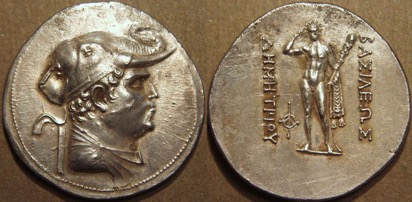
\includegraphics[width=.6\linewidth]{Raza-Figure01}
	\caption{Demetrius I. On left, obverse design representing king wearing elephant headdress, and on the reverse on right, Heracles crowning himself with a diadem.
		{\normalfont\scriptsize \\ \copyright\ by \cite{Coin}, image used with permission}}
	\label{fig:Raza-Figure01}
\end{figure}
%\end{wrapfigure}

The elephant is the most widely recurring animal on the coins \parencite[383--384]{Bopearachchi1991}.
It was considered emblematic of kingship on account of its physical stature and strength,
while its fondness for bathing and the use of the trunk to spray water led to an association with fertility and sky deities,
among others \parencites[15--19]{Gupta1983}[156]{Iossif2010}.
The first coin type under consideration is the elephant headdress.
This refers to the representation of the ruler on the obverse in a headdress resembling the head of an elephant.
Three Greco-Bactrian and Indo-Greek kings issued coins of this type, but discussion has centred on the coins issued by Demetrius I
(c. 200-185\BC) (see \cref{fig:Raza-Figure01}), the ruler to whom scholars attribute the first wave of Greco-Bactrian conquests in India
\parencites[47--48]{Bopearachchi2011}[17--18]{Kalita1997}.
Explanations for the symbolic meaning and function of the elephant headdress has centred on Greek precedent,
namely, the iconography of Alexander the Great.
Patterned on the lion scalp of Heracles, Alexander had been represented wearing the elephant headdress on the coins of Ptolemy,
his general who became king of Egypt \parencite[21--31]{Lorber2012}.
It is thought that Ptolemy was representing Alexander as an elephant slayer, and thus symbolically alluding to conquests in India,
the elephant being a personification of the country \parencites[50]{Curtis2007}[335]{Green1993}[104--105]{MacDowall2007a}.
Alexander himself had issued the so-called ‘Elephant Medallion’ coins, which represent his triumph over the elephants of the Indian
king Porus, and hence symbolically over Indians \parencite[151--152]{Holt2003}.
Consequently, the elephant headdress is thought of as Greek triumphalism, the symbol of their right to rule by victory over Indians.
In the words of one scholar, the symbolism was one of “massacre d’elephant” \parencite[232, 492]{Widemann2009}.
Such an interpretation would support negative assessments of Greek engagement with local traditions.
The elephant was associated with various Indian divinities, including the sky god Indra, and its representation as a hunting trophy
would be analogous to the Persian king Cambyses’ alleged violation of the Apis Bull in Egypt \parencite[15--19]{Gupta1983}.

However, the interpretation of the elephant headdress as a symbol of conquest is at odds with the chronology.
Demetrius’ elephant headdress coins appear from the very outset of his reign, before the new king would have had the chance
to invade India \parencite[157]{Holt2012}.
The presupposition that the elephant headdress must refer to military triumphs has consequently led to attempts to revise the dates
for Demetrius’ campaigns.
One suggestion is that Demetrius invaded India during the reign of his father Euthydemus I (c. 230--200\BC).
The Kuliab inscription from Tajikistan hails Demetrius as Kallinikos, the glorious victor, while Euthydemus is honoured as king,
and this has been taken to refer to victories gained by Demetrius in India under his father \parencite[104--105]{MacDowall2007a}.
However, it has been pointed out that the inscription could have been alluding to Euthydemus and Demetrius thwarting the Seleucid king
Antiochus III, who had unsuccessfully invaded the Greco-Bactrian kingdom in 209--206\BC \parencite[48]{Bopearachchi2007}.
Alternatively, it is possible that the inscription alluded to Greco-Bactrian expansion into Aria (modern Herat),
one of the satrapies north of the Hindu Kush that Seleucus had handed over to the Mauryan king Chandragupta in exchange for elephants.
Polybius locates the first battle between Antiochus and Euthydemus near the Arius River inside Aria in 209\BC,
and from this, it might be surmised that the Greco-Bactrians had reoccupied the province under Euthydemus.
Demetrius might have participated \parencite[48]{Lerner1999}.

One final argument for revising the date of the Indian campaigns is that Strabo identifies Demetrius as the son of
Euthydemus when describing the Greco-Bactrian conquests \parencite[183]{Holt1999}.
Strabo’s wording has been taken to mean that Euthydemus was alive and reigning at the time Demetrius invaded India \parencite[157--158]{Holt2012}. 
However, Strabo was summarising another writer, Apollodorus of Artemita, and his own work was a geographic treatise light on chronology.
Strabo writes as if the conquests of Demetrius were concurrent with Menander I (c. 165/155--135\BC), who was a later Indo-Greek king,
but this became the impression of early scholars such as Tarn \parencite[144]{Tarn1951}.
Overall, it is difficult to allow for Greco-Bactrian expansion into India (south of the Hindu Kush mountains in modern Afghanistan)
under Euthydemus.
The war with the Seleucids had been detrimental to royal power and Euthydemus had to hand over his elephants in exchange for
sovereignty \parencite[130]{Holt1999}.
In addition, nomadic incursions had been troubling the Greco-Bactrian kingdom.
Polybius says that the joint threat posed to Antiochus and Euthydemus had been a major impetus to peace.
Significantly, the northern province of Sogdiana was evidently lost to the Greco-Bactrians at the time of Antiochus’
three-year long siege of the royal capital at Bactra in 208--206\BC \parencite[135]{Holt1999}.
The Greco-Bactrians were consequently preoccupied with the defense of the kingdom, if not attempting to recover Sogdiana,
as well as generally attempting to restore royal authority in the aftermath of the Seleucid invasion
\parencites[60--61]{Lerner1999}[236]{Widemann2000}.

If Demetrius won victories in India under his father, it would have been later, in the second century\BC.
This would require revising the accepted dates for Euthydemus.
One argument is that the Indo-Greek era beginning in 186/185\BC was inaugurated by Demetrius to mark his ascension as king
and thus allowing for a period of campaigning under his father in the second century \parencite[104--105]{MacDowall2007a}.
However, the traditional date for the Indo-Greek era is only an estimate, and some scholars have argued that its inception
should be pushed to 175/174\BC \parencites[48]{Bopearachchi2011}[210--211]{Falk2009}.
If accepted, it would be difficult to revise the dates for Demetrius and Euthydemus as far forward as some have argued,
especially since a new generation of rulers appear in the numismatic record from the 180s \parencite[505]{Jakobsson2009}.
Moreover, Hellenistic royal eras generally began with the reign of the first king of the dynasty,
and it is improbable that Demetrius – if he did inaugurate the Indo-Greek era – would have overlooked his father \parencite[506]{Jakobsson2009}.
Certainty, Euthydemus had established the rule of his dynasty, and his prestige is evident from the superlatives accorded to him
in the Kuliab inscription.
Demetrius also struck commemorative coins, hailing his father as Euthydemus Megas, the Great \parencite[111]{Hollis2011}.
A later ruler who considered Demetrius the founder of Greek rule in India would be a more probable candidate for the establishment
of the Indo-Greek era.
Royal epochs could be, and often were, instituted retrospectively for political purposes \parencite[506]{Jakobsson2009}.
The identity of the king responsible remains uncertain, but if the Indo-Greek era did begin in 186/185\BC, and if the inception
of the era did allude to a date in Demetrius’ career, it should be associated with the campaigns in India.
That Demetrius was important to later rulers is evident from his appearance on the commemorative or ‘pedigree’ coins struck by
the Indo-Greek kings.
Significantly, Demetrius was given the posthumous epithet of Aniketos, the invincible,
suggesting that it was his military prowess for which the later Indo-Greeks remembered him \parencite[48]{Bopearachchi2011}.

Admittedly, the proposed reconstruction is hypothetical, and the date of Demetrius’ campaigns cannot be fixed with any certainty.
The campaigns might have taken place earlier, and if so, it would be possible to add a few years to Euthydemus’ reign
to create a window for Demetrius to campaign under his father at the turn of the century,
and without causing a major chronological crux.
One scholar thus places Euthydemus’ death in 195\BC, presumably allowing for a period of recovery from the external invasions,
following by expansion in c. 200--195\BC\ \parencite[111]{Hollis2011}.
However, this reconstruction might understate the nomadic threat.
Beginning in c. 200\BC, the archaeological evidence indicates the construction of several new fortifications in the Central Asian
frontiers of the Greco-Bactrian kingdom, as well as in the city of Ai Khanoum \parencite[135]{Holt1999}.
This suggests that the nomads were still a major concern to the Greco-Bactrians, and even if Euthydemus had lived up to 195\BC,
expansion into India at this time seems improbable.
The campaigns would be best dated towards the middle and end of Demetrius’ reign.

Thus, it is difficult to read Demetrius’ elephant headdress as a symbol of victory.
In fact, the headdress was not patterned on the elephant scalp worn by Alexander,
the possible emulation of which has guided the traditional interpretation.
Maritz and Smith have pointed out that the headdress worn by the Greco-Bactrian and Indo-Greek kings is rendered on the coins
as a military helmet, as opposed to the elephant hide draped around Alexander’s head \parencites[48]{Maritz2004}[63]{Smith1986}.
Significantly, the helmet variant of the elephant headdress is worn only by these kings, while other Hellenistic rulers
represented themselves in headdresses following the convention of the animal scalps of Heracles and Alexander.
Furthermore, the origin of the elephant headdress need not be necessarily linked to India.
Over their history, elephants had become a symbol of Seleucid royal power, and there might have been a similar development in
the Greco-Bactrian kingdom.
Firstly, there is the evidence of Greco-Bactrian phalarae, which represent Indian war elephants prominently \parencite[1206--1211]{Bannikov2013}.
A phalara was a metal disk worn as decorations on breastplates and horse harnesses.
It is thought that the elephant phalarae were worn by the Greco-Bactrian cavalry, and possibly the elephant corps as well 
\parencites[1206--1211]{Bannikov2013}[10]{Pfrommer1993}[588]{Treister1999}.
In addition, it is suggested that the Greco-Bactrian infantry might have also worn helmets patterned on the elephant \parencite[163--180]{Abdullaev1995}.
Royal self-presentation in an elephant helmet would thus fit into the context of the military iconography of the Greco-Bactrians.

Demetrius would have been associating with the visually most impressive element of the Greco-Bactrian army,
as well as a Hellenistic symbol of royal power.
Secondly, while Greeks might have seen the elephant headdress as an allusion to Alexander, such attires were also traditional to Bactria.
Local aristocrats were buried in headdresses adorned with horns and feathers,
and it was thought that the wear of such attire could transfer the power of the animal to humans \parencite[215--226]{Lerner2009}.
Demetrius thus might have been expressing royal power in a Greek context as a successor to Alexander,
and as an owner of mighty war elephants, as well as in a local context by symbolically claiming the power of the elephant.

\begin{figure}[!htb] %Figure 2
	%\begin{wrapfigure}{O}{0.5\textwidth} 
	\centering
	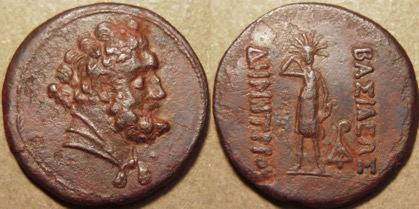
\includegraphics[width=.6\linewidth]{Raza-Figure02}
	\caption{Demetrius I. On left, obverse design with bust of Heracles, and on the reverse on right, Artemis with a radiate halo. 
		{\normalfont\scriptsize \\ \copyright\ by \cite{Coin}, image used with permission}}
	\label{fig:Raza-Figure02}
\end{figure}
%\end{wrapfigure}

It is interesting to note that the reverse design of the elephant headdress coin type depicts the coronation of Heracles (see \cref{fig:Raza-Figure01}),
who, in Greek tradition, became the king of Bactria and India \parencites[70--80]{Bukharin2004}[140]{Stanco2012}. %%% Stanco2012 or Stanco2015?
Thus, the coins draw attention to royal sovereignty, and in a clearly Greek context.
Yet another coin type of Demetrius depicts a bust of Heracles on the obverse, while Artemis appears with a radiate halo on the reverse,
evidencing her approximation to Anahita —a regal deity of the Iranians and cult goddess of Ai Khanoum (see \cref{fig:Raza-Figure02})
\parencite[242]{MacDowall2007b}.
This suggests that Demetrius’ self-presentation took into account his Bactrian subjects.
There would have been good cause for this, with the Greco-Bactrian army being multiethnic in composition.
The elephant phalarae, for example, depict Greek and Bactrian soldiers on battletowers strapped to war elephants led by Indian mahouts
\parencites[10]{Pfrommer1993}[588]{Treister1999}.
It is suggestive that these phalarae were worn as decorations by the Greco-Bactrian cavalry, itself a multiethnic force comprising
Greeks and Bactrians, among others \parencite[50--51]{Lerner1999}.
Since the elephant headdress originated before the invasion of India, the coin type might be seen as an expression of royal power
in a distinct Greco-Bactrian context, influenced in part by Greek tradition, and in part by that of Bactria.

\begin{figure}[!htb] %Figure 3
	%\begin{wrapfigure}{O}{0.5\textwidth} 
	\centering
	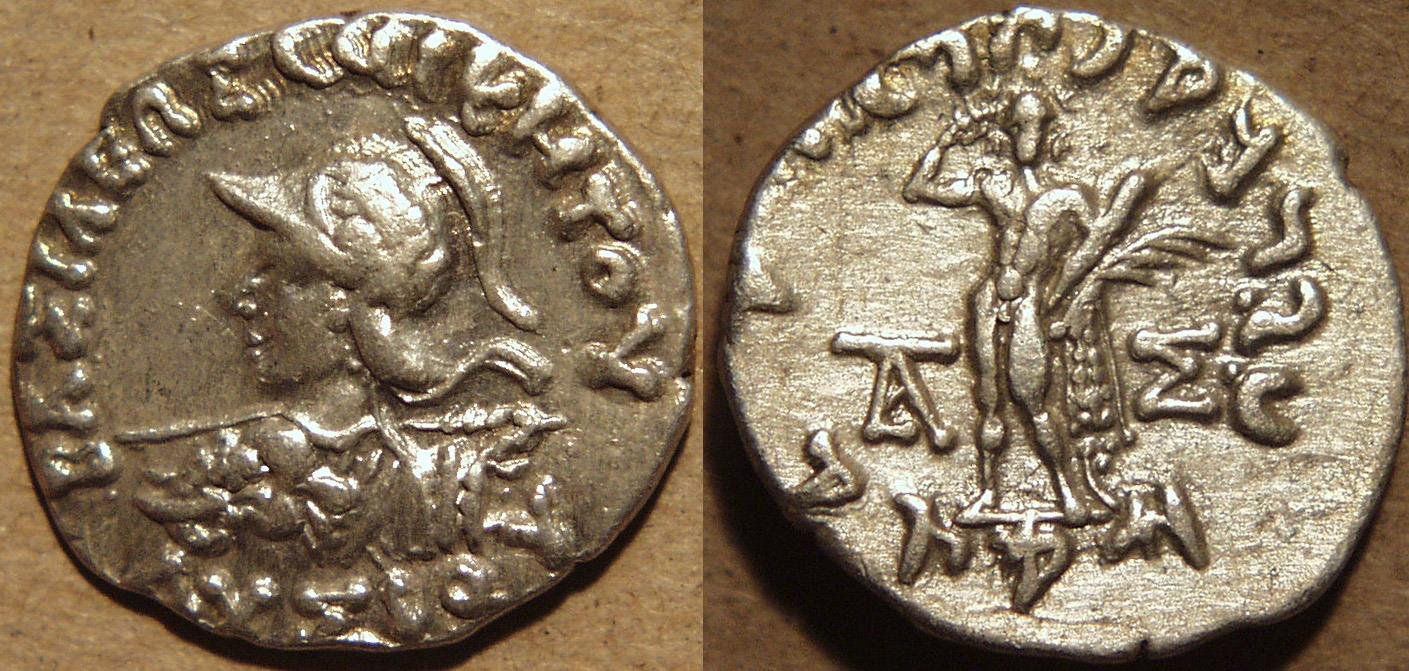
\includegraphics[width=.6\linewidth]{Raza-Figure03}
	\caption{Lysias. On left, obverse design representing king wearing elephant aegis on his left shoulder. Note the elephant’s protruding tusks and the trunk tapering downwards. On the reverse on right, Herakles crowning himself with a diadem. 
		{\normalfont\scriptsize \\ \copyright\ by \cite{Coin}, image used with permission}}
	\label{fig:Raza-Figure03}
\end{figure}
%\end{wrapfigure}

After Demetrius, the elephant headdress coin type was next issued by Lysias (c. 120--110\BC), an Indo-Greek king who ruled
territories near Arachosia and Paropamisade in modern Afghanistan. 
Unlike Demetrius, nothing is recorded of Lysias in the literary sources, but it has been supposed that his coins allude to
victories in India as well \parencite[107]{Widemann2003}.
The same assumption applies to Lysias’ elephant aegis coin type. 
While Indo-Greek kings generally wear on the shoulder an aegis decorated with the traditional head of the Gorgon, Lysias is
represented in an armour patterned on the head of an elephant, while brandishing a spear in one hand (see \cref{fig:Raza-Figure03}) \parencite[71]{Whitehead1970}. 
It has been thought that this represents a hunting trophy patterned on the animal skins worn by Alexander and Heracles,
symbolising Lysias’ power as an elephant slayer, and one scholar thus writes that the king substituted the traditional aegis with
an elephant scalp \parencite[341]{Cribb2011}. 
Moreover, the self-presentation of Lysias in the act of hurling a spear call to the mind the Greco-Macedonian ideology of
doriktetos chora, ‘by the spear’, that is to say, the right to rule by conquest \parencite[27]{Billows1995}. 
Yet, this interpretation is at odds with Lysias’ association with another king, Antialcidas (c. 115-95\BC). 
Lysias and Antialcidas were joint kings, or at least, close allies. 
Both rulers share monograms, the marks made on coins by minting officials, indicating that they shared access to the same mints. 
Furthermore, Antialcidas and Lysias struck a series of so-called ‘mule coins’, with both their names and titles placed opposite to
one another \parencite[121]{Mairs2014}.

\begin{figure}[!htb] %Figure 4
	%\begin{wrapfigure}{O}{0.5\textwidth} 
	\centering
	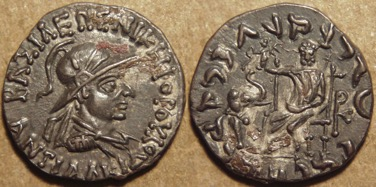
\includegraphics[width=.6\linewidth]{Raza-Figure04}
	\caption{Antialcidas. On left, obverse design with bust of king, and on the reverse on left, representations of Zeus and Nike. Note the protome of an elephant trumpeting.
		{\normalfont\scriptsize \\ \copyright\ by \cite{Coin}, image used with permission}}
	\label{fig:Raza-Figure04}
\end{figure}
%\end{wrapfigure}

Generally, Antialcidas associated the elephant closely with Zeus. The reverse design of one coin type depicts Zeus enthroned,
holding sceptre in one hand, and supporting the goddess Nike with the other.
Nike herself holds a wreath symbolising victory.
At the bottom right, an elephant protome is depicted, with its trunk raised towards Zeus (see \cref{fig:Raza-Figure04}).
This is interesting because the trunk of the elephant, when raised upwards, symbolises a salute \parencite[33--34]{Whitehead1970}.
If so, the elephant might be seen as saluting Zeus as its master.
The portrait of Antialcidas appears on the obverse, associating the king with the imagery. 

\begin{figure}[!htb] %Figure 5
	%\begin{wrapfigure}{O}{0.5\textwidth} 
	\centering
	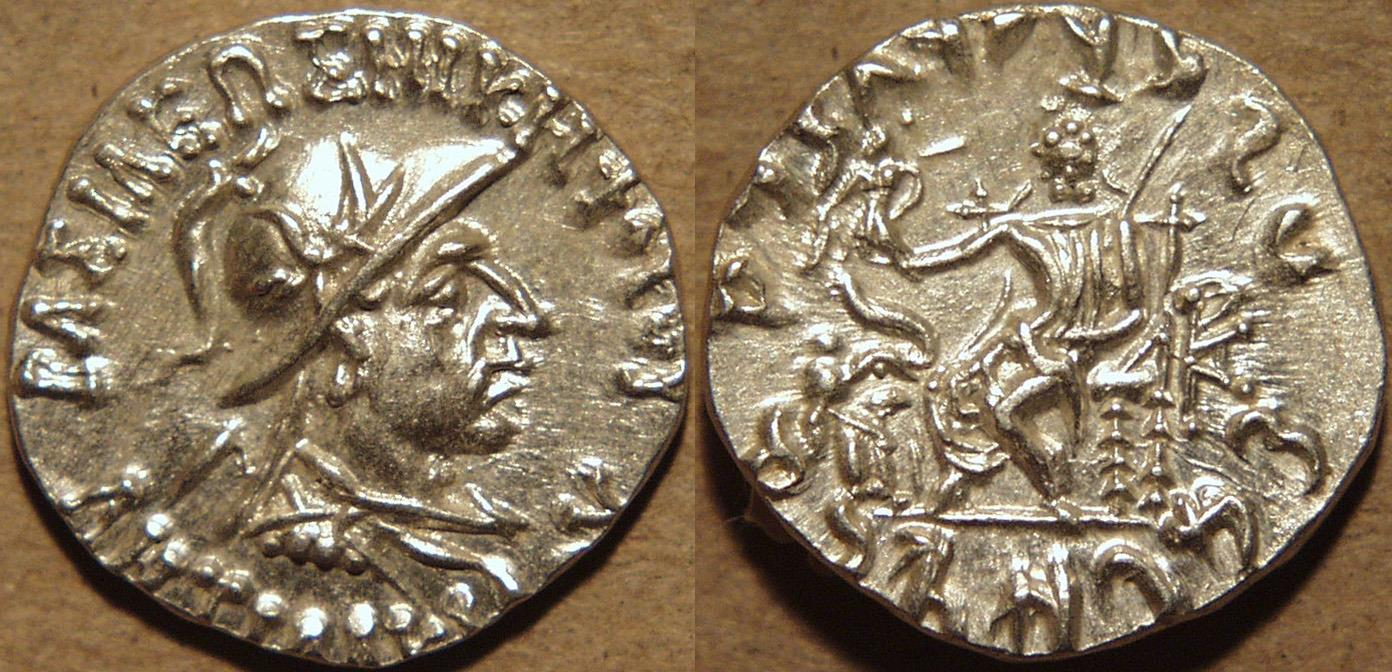
\includegraphics[width=.6\linewidth]{Raza-Figure05}
	\caption{Antialcidas. On left, obverse design representing the king brandishing spear. Note the aegis on left shoulder. On the reverse on right, Zeus striding besides elephant. Nike holding wreath stands on top of elephant’s head.
		{\normalfont\scriptsize \\ \copyright\ by \cite{Coin}, image used with permission}}
	\label{fig:Raza-Figure05}
\end{figure}
%\end{wrapfigure}

Another coin type depicts the king on the obverse, while Zeus appears on the reverse, striding besides an elephant with sceptre in hand. 
Nike stands on top of the elephant’s head and holds in hand a wreath symbolising victory (see \cref{fig:Raza-Figure05}) \parencite[27]{Narain1991}. 
This type explicitly identifies the elephant with Zeus. 
The significance of Zeus’ association with the elephant is that Indians would have recognised the figure of a divinity
– holding sceptre and physically dwarfing an elephant – but not necessarily Zeus. 
Rather, it is possible that the figure with the elephant might have been recognised as Indira,
the Indian sky god with whom the elephant was also associated \parencite[247]{MacDowall2007b}. 
It is suggestive that the coins of the Indo-Greek king Antimachus I (c. 174--165\BC) associated the elephant with a winged thunderbolt,
the iconic attribute of both Zeus and Indra (see \cref{fig:Raza-Figure06}) \parencites[242]{MacDowall2007b}[260]{Narain2003}.
Significantly, the final king to represent himself in an elephant headdress, Demetrius III (c. 100\BC),
deployed the winged thunderbolt as the reverse design \parencites[17--18]{Kalita1997}[362]{Sircar2008}.
This suggests that the wear of elephant headdresses might have become associated with Zeus by this time. 
If Lysias and Antialcidas were closely related, it would be difficult to reconcile the elephant’s proximity to Zeus on the one hand,
and the possible predatory meaning ascribed to the symbolism on the other.

\begin{figure}[!htb] %Figure 6
	%\begin{wrapfigure}{O}{0.5\textwidth} 
	\centering
	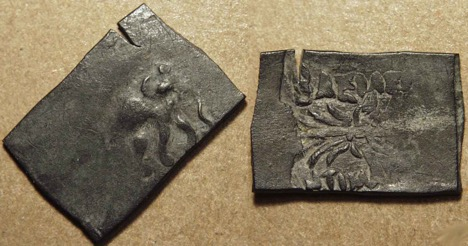
\includegraphics[width=.6\linewidth]{Raza-Figure06}
	\caption{Antimachus I. On left, the obverse design representing elephant walking, and on the reverse on right, a winged Thunderbolt.
		{\normalfont\scriptsize \\ \copyright\ by \cite{Coin}, image used with permission}}
	\label{fig:Raza-Figure06}
\end{figure}
%\end{wrapfigure}

Thus, it seems probable that Lysias’ elephant armour represented an aegis, meant to invoke the protection of Zeus and Indra \parencite[71]{Whitehead1970}.
Interestingly, Indra is described in the Vedas as being “clothed in might like an elephant”, drawing a parallel to
the symbolic function of the elephant headdress and armour of the Indo-Greek kings \parencite[22]{Gupta1983}. 
An objection could be that, while the Indo-Greeks might have associated Zeus with the elephant,
it need not have necessarily denoted a connection to Indra. 
On Seleucid coinage, Greek divinities such as Zeus appear in an elephant driven chariot,
reflecting the exalted status of the royal war elephants as divine mounts \parencite[254--270]{Alonso2013}. 
However, in the case of the Indo-Greeks, there is cause to believe that the Greeks associated the elephant with Indra. 
Antialcidas is on historical record as the Indo-Greek ruler who sent the ambassador Heliodorus to the court of the Indian king,
Bhagabadra, in Vidisha (in modern Madhya Pradesh, India). 
Heliodorus left behind an inscription in the area, professing to be a devotee of the Indian deity, Vasudeva,
who was one of the manifestations of the supreme divinity of the Vaishnavite cult, Vishnu.
Most significantly, Heliodorus designates the structure set up in his name as the ‘Garud pillar’,
alluding to Garuda, the mythical sacred bird of Vishnu. 
It is thought that the structure originally supported images of Garuda \parencite[126--127]{Mairs2014}. 
Besides indicating that some Greeks actively took part in local cults, the inscription suggests that they were aware of
the iconographic symbols of local divinities. 
Thus, it is possible that the Indo-Greek kings were not ignorant of the significance of the elephant to Indra,
and deployed elephant imagery as an all-encompassing political symbol. 
If so, the elephant headdress and elephant aegis suggests an Indo-Greek royal conception of power that extended beyond
their Greek heritage, incorporating local Indian traditions as well.

\begin{figure}[!htb] %Figure 7
	%\begin{wrapfigure}{O}{0.5\textwidth} 
	\centering
	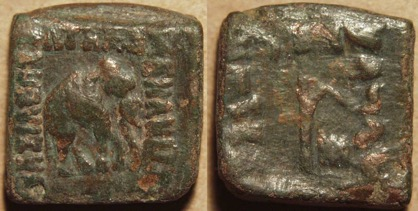
\includegraphics[width=.6\linewidth]{Raza-Figure07}
	\caption{Menander I. On left, the obverse design representing elephant walking, and on the reverse on right, an elephant goad.
		{\normalfont\scriptsize \\ \copyright\ by \cite{Coin}, image used with permission}}
	\label{fig:Raza-Figure07}
\end{figure}
%\end{wrapfigure}

The last elephant coin type under consideration is the ‘elephant and goad’.
This refers to representations of the elephant on the obverse and an elephant goad on the reverse (see \cref{fig:Raza-Figure07}). 
The coin type was issued by only one king, Menander, who ruled an extensive empire centred on the Punjab in modern Pakistan and India. 
Menander is generally considered the greatest Indo-Greek ruler and his coins are the most numerous from those yet recovered \parencite[14--17]{Bopearachchi1993}.
Furthermore, Menander is the only Indo-Greek ruler to have been preserved in both Indian and classical sources. 
The Buddhist text Milindapanha purports to record the dialogue between Milinda, or Menander, on the one hand,
and the Buddhist monk Nagasena on the other. 
The text portrays Menander as a wise philosopher king and convert to Buddhism who gave up his throne to retire to an ascetic life
\parencite[14--17]{Bopearachchi1993}. 
Classical sources give a different perspective.
Plutarch writes that Menander was celebrated for his rule, but that he died in camp, that is to say, while on a military campaign. 
Strabo adds that Menander was among the most successful Greek generals in the east and that he possibly conquered even more
Indian peoples than Alexander the Great \parencite[180, 183]{Holt1999}.

The symbolic meaning and function of Menander’s elephant and goad type has not attracted much comment. 
For comparison, the elephant goad appeared on Seleucid coinage, held in hand by a turbaned figure on the obverse of one coin type.
An elephant is depicted on the reverse. 
It has been argued that the turbaned figure represents Dionysus, who, in Greek tradition, conquered India,
and taught the Indians to wear turbans.
Consequently, the coin type has been taken to represent Dionysus in his aspect as the conqueror of India,
the goad symbolising his dominion over the elephant, and hence, of India \parencite[147--164]{Iossif2010}.
An interpretation that sees the Indo-Greeks as failing to engage with local traditions might thus be that Menander was
symbolising his power as a Greek king over the land of the elephant, India.
Interestingly, despite his reputation as a wise philosopher king in Indian tradition, the military dimension of Menander’s
career has been emphasised in scholarship. 
This arguably reflects the weight given to classical sources.
One scholar counts Menander among kings like the Greco-Bactrian Eucratides I (c. 170-145\BC), who, according to Justin,
had “bled Bactria to death” through his frequent wars \parencite[128]{Holt2005}. 
Another scholar summarily dismisses Menander’s reputation as a benign ruler and emphasises his ‘warlike’ tendencies instead \parencite[15--16]{Widemann2007}.

The elephant and goad type is significant because it might provide an insight into Menander’s legendary reputation.
Firstly, elephants had more than just a military role in Indian political tradition.
As the sacred animal of Indra, the sky god, elephants were associated with rainfall in various legends \parencites[19]{Gupta1983}[37--43]{Srivastava1989}.%Srivastava1989 or Srivastava1999 ?
One recurring story was that elephants were originally clouds, cursed to wander the earth, 
and thus indirectly responsible for rain when their brethren would come visit them \parencite[38--39]{Gonda1966}. 
Another was that Indra’s sacred elephant, Airavata, was directly responsible by sucking up water from the underworld for
Indra to dispense from the sky above \parencite[23--24]{Gupta1983}. 
In time, the Buddha, too, became associated with the elephant and rainfall \parencite[23--24]{Gupta1983}. 
Consequently, elephants were the symbols of fertility par excellence, and it was the duty of the king to maintain them in
the royal stables for the purpose of ensuring the timely arrival of the monsoon. 
The bond between king and elephant was such that the animal was referred to as the ‘king’s cloud’, and,
as one of the seven ratnas or jewels of the rightful Indian monarch \parencites[38--39]{Gonda1966}[107]{Zimmer2015}.
The goad, as the instrument used by elephant trainers or mahouts to train and control elephants,
acquires royal significance in that context.
The coin type might have signified Menander’s possession of elephants and hence an acknowledgment of his royal duty of maintaining
the fertility of the kingdom.

The elephant and goad coin type might also have had connotations of justice.
The purpose of the goad had been to tame, control, and direct the elephant. 
This involved not only encouraging the elephant to move forward in battle, but also, when necessary, to retrain it \parencite[66--67]{Trautmann2015}. 
The highly symbolic nature of the goad as an instrument of control led to its association with law. 
Nirankusa, a word derived from ankusa, meaning goad in Sanskrit, came to refer to people who did not follow social norms and rules. 
Thus, the Indian elephant god Ganesha, who possibly originated during the Indo-Greek period, 
held the goad as a symbol of his power to restrain the forces of evil \parencites[96]{Alter2004}[55]{Dhavalikar1991}.%Dhavalikar1991 or Dhavalikar1981 ??
Similarly, among the sayings of the Buddha, the elephant and goad parable was central. 
The love and wisdom of the Buddha was said to have tamed the wicked elephant Nalagiri, 
much like a mahout tames his elephant with the goad \parencite[96]{Dhammika2005}. 
Thus, it might not be coincidental that Menander was remembered as a good king. 
The reading of the coin type would support Menander’s engagement with local political traditions and kingship practices,
and account for his reception in Indian tradition. 
Admittedly, it is quite possible that Menander was also representing his military power through the elephant. 
Elephants remained an important part of the Indo-Greek armies, and as a symbol of control,
the goad might have represented Menander’s possession of the powerful animals.
Alexander’s ‘Elephant Medallion’ coins had evidently represented Porus wielding a goad on the back of an elephant,
indicating the king’s control of the animal \parencite[204--205]{Stewart1993}.
Furthermore, Strabo emphasises Menander’s reputation as a warrior, as opposed to his engagement with local traditions \parencite[644]{Mairs2014}.
This would be explainable by the fact that the elephant symbolism was multivalent. 
A Greek might have seen in the symbolism an expression of Hellenistic military power,
while an Indian might have considered the elephant and the goad in context of local traditions. 
The point is that the coin type would have resonated in both Greek and local contexts.

In conclusion, elephant symbolism on the coins of Greco-Bactrian and Indo-Greek kings was intended to legitimise
royal authority in a cross-cultural context, accommodating the political traditions and kingship practices of Bactria and India.
The view that the Greco-Bactrians and Indo-Greeks did not engage with local ruling traditions is not borne out by the coins.
The picture that emerges supports the recent literature that emphasises the cosmopolitan conception of royal power in
the Hellenistic kingdoms \parencite[11]{Strootman2014}.
However, a Hellenocentric approach has obscured the cross-cultural significance of the elephant imagery,
leading to the view that the Greco-Bactrian and Indo-Greek rulers confined themselves to Greek ruling traditions. 
When studying the coins, scholars should take note to consider not only the Greek context,
but also the possible local significance of the iconography. 
Through consideration of local contexts, scholars will be able to gain a better understanding of how Hellenistic kings
established and maintained their power over diverse, multiethnic populations.
\IJSRAclosing%<<<< DO NOT change this line
\end{document}
